\documentclass[letterpaper]{article}
\usepackage[top=3cm, bottom=3cm, left=3.85cm, right=3.85cm]{geometry}
\usepackage{graphicx}
\usepackage[utf8]{inputenc}
\usepackage[english]{babel}
 \usepackage{notoccite}
\usepackage[backend=bibtex,style=numeric,sorting=none]{biblatex}
\addbibresource{beam_lightning.bib}
\graphicspath{ {./images/} }

\begin{document}
 
\title{Beam Lightning Network Position Paper}
\date{\today\\V 1.0}
\author{Fabian Jahr, for Beam}
 
\maketitle

\section{What is the Lightning Network?}
 The Lightning Network is a second layer scaling solution for blockchains. It enables extremely fast and cheap transfers of value off-chain that can be settled on-chain at any moment. At the same time, the Lightning Network does not sacrifice trustlessness, security or decentralization. To achieve this, the Lightning Network is based on the broader concept of payment channels, which are implemented through a limited set of smart contracts.

\begin{figure}[h]
	\centering
	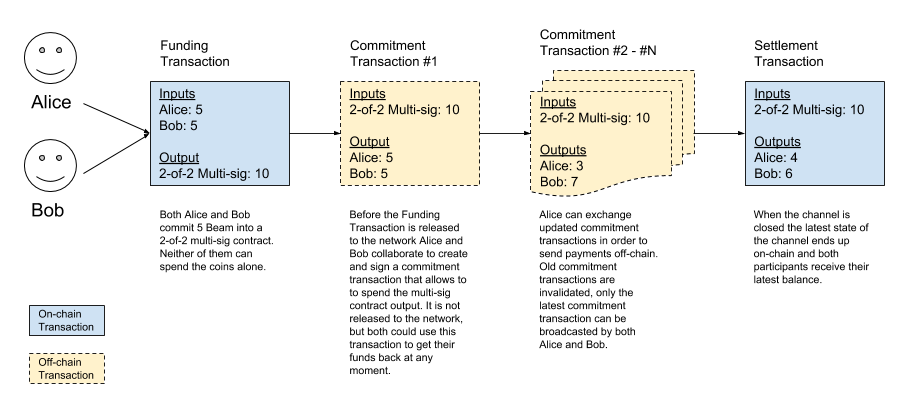
\includegraphics[width=\textwidth]{payment_channel_high_level}
	\caption{High level mechanics of a payment channel between Alice and Bob. Inspired by figure 12-4 of Mastering Bitcoin.}
\end{figure}

Off-chain payment channels are not a new idea. The concept was already a topic of discussion in the Bitcoin community when Satoshi was still around, although his original idea of payment channels was flawed \cite{satoshi}. Several ways of constructing payment channels were explored by researchers over the year until Joseph Poon and Thaddeus Dryja presented their version of payment channels, called the Lightning Network, in 2015 \cite{lightning}. Their findings, along with the support of several other researchers, was the breakthrough that led to the state of the Lightning Network that we can use on Bitcoin mainnet today. 

At the time of writing the Lightning Network on Bitcoin mainnet is counting 5,700 active nodes, 22,000 public channels and a capacity of over 600 Bitcoin (2M USD) \cite{stats}. As the network only got started little more than a year ago, these numbers are clearly impressive. While there are still challenges ahead for the Lightning Network itself, especially making it more robust and user-friendly, the Team of Beam has built a strong belief that Lighting Network has already proven to be the currently best choice of a scaling solution for blockchains today and thus worth a significant investment of our resources.

\section{Why Lightning Network on Beam?}
At first glance users may ask if a scaling solution is really necessary on Beam: after all, Beam has a block time of only one minute while Bitcoin only forms a block only every 10 minutes. Why is there still the need for a Lightning Network if Beam is already “ten times faster”?

To begin with, faster block time does not necessarily mean faster payment confirmation. While in Bitcoin it is generally advised to wait for 6 confirmations (6 blocks mined on top of the transaction) for a serious transaction to be considered fully settled, users of Beam may rather want to wait for a period in the realm of up to 60 confirmations to get the same level of confidence in the received payment, especially while the network is still young and hashpower is comparably low.

Furthermore, there are many use cases that we want to use digital cash for, where there is only minimal tolerance for wait times. It may be ok to wait for a couple of minutes when you are paying for beers at a local bar and you are not in a hurry to leave. But think of just quickly grabbing a drink from a vending machine while you are trying to catch your train or paying at a busy checkout with a long queue of other nervous customers behind you. For Beam to take over these use cases as well, we clearly need to achieve “Visa level” speed of payments, if not even beat it. Trials have shown that the Lightning Network is able to achieve payment speeds that make the payment experience as quick and easy as a credit card payment which make it one of the cornerstones along the way to achieve mainstream adoption of cryptocurrencies in general.

Last but not least, Beam’s transaction capacity per second is currently about three times that of Bitcoin, which is a nice increase. But it is still not nearly at a level that would allow for “Visa level” transaction throughput. If we can achieve a user experience that enables mainstream adoption as described in the previous paragraph, we also need the transaction capacity that is able to carry it. A second layer solution like Lightning Network allows transaction capacity to scale orders of magnitude without the need to extend the base layer of the blockchain. Mainstream adoption would simply not be feasible without it.

\section{Lightning Network challenges on Beam}
There are many differences between MimbleWimble and Bitcoin, and some of these differences are posing issues for the Lightning Network integration of Beam. Some, like the interactive nature of transaction construction, luckily solve themselves. Lightning nodes need to be reliably online most of the time anyway. The major issue, however, is the lack of scripts in the MimbleWimble protocol. 

This is where the magic of scriptless scripts comes in, a concept introduced by Andrew Poelstra along with his initial thoughts on MimbleWimble itself \cite{poelstra}. Scriptless scripts allow for the construction of smart contracts without the usage of a scripting language by encoding the script into a signature instead. They are blockchain-agnostic, the only major requirement is the use of Schnorr signatures. Scriptless scripts are a part of Beam today and as such have already provided solutions for many of the requirements that the Lightning Network is built on.

Lightning Network funding transactions are essentially a 2-of-2 multi-sig transaction, which is possible in Beam through the collaborative construction of the transaction demonstrated in our documentation as part of Atomic Swaps for example \cite{swap}. The main difference is that the number of messages going back and forth between the peers is slightly increased due to the difference in the underlying MimbleWimble protocol.

The construction of Hash Time Locked Contracts, the core concept of the Lightning Network, requires two more smart contract schemes: hashlocks and relative timelocks. Hashlocks have been a part of the base protocol of Beam from the start \cite{transaction}. But while Beam has implemented absolute timelocks, relative timelocks are not available yet. Thankfully, members of the MimbleWimble Mailing List, mainly consisting of members of the Grin development team, have identified a solution to this issue already which we agree with and plan to implement in Beam as well \cite{contracts}.

But how do we chain these concepts together without a script? Where there are multiple execution paths of a script in Bitcoin, in MimbleWimble we will need to use multiple transactions that build on top of each other. The spending requirements of these transactions will work together to form the same construct as HTLCs in Bitcoin and the participants of a payment channel will collaborate to construct these different transactions. This, again, leads to an increase in messages being sent between the participants of a channel, but the gain is more than worth it.

\begin{figure}[h]
	\centering
	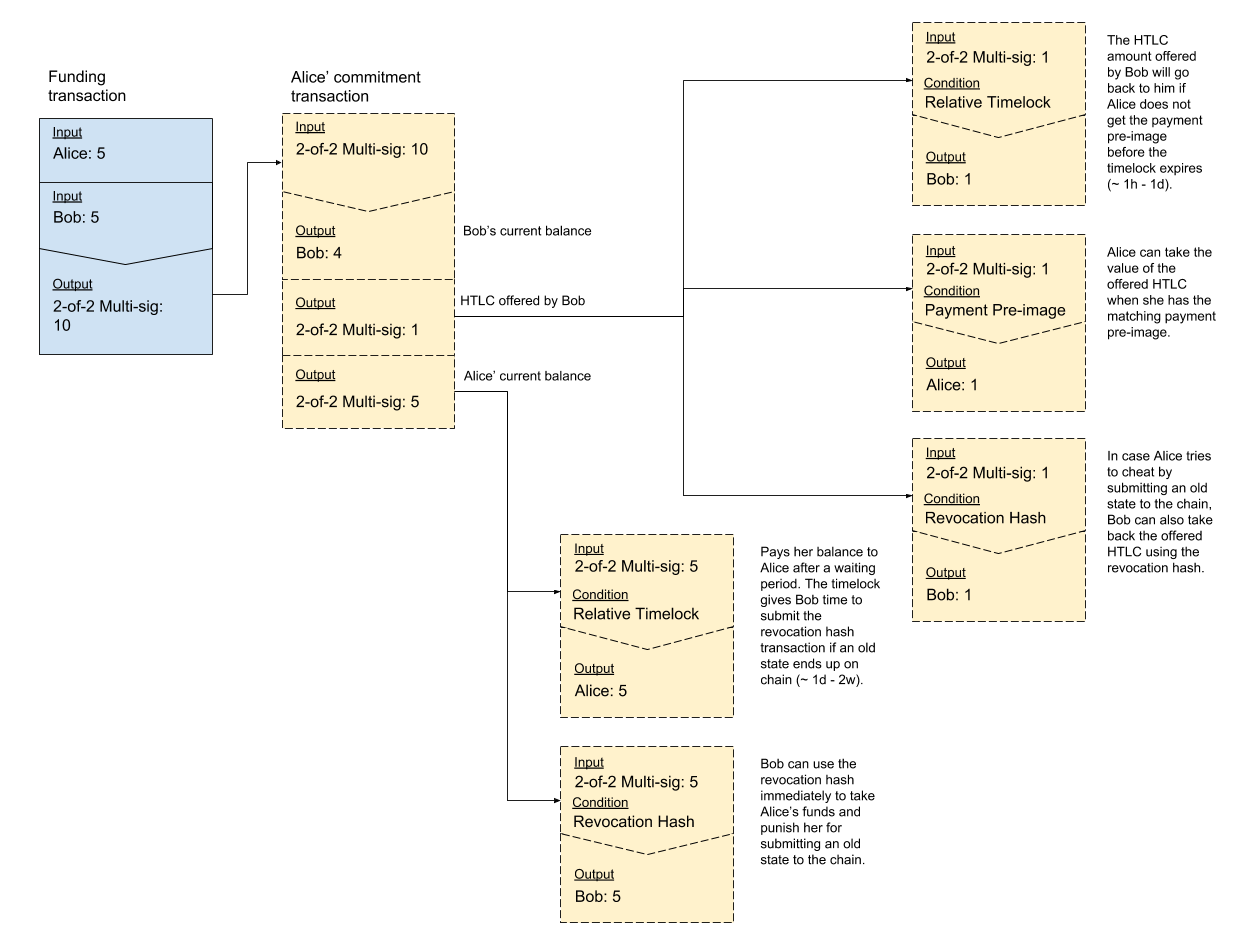
\includegraphics[width=\textwidth]{lightning_mw_transactions_htlc}
	\caption{Exemplary transaction structure on Alice’ side of a Lightning Network payment channel on MimbleWimble.}
\end{figure}

\section{Project Roadmap}
Throughout the past couple of weeks, the development team of Beam has been researching the necessary requirements for a Lightning Network integration with Beam. For that purpose, we are working on a fork of the Lightning Network RFCs that document the adaptations to the protocol on a high level to work with any MimbleWimble implementation \cite{lmw}.

For Beam specifically, the next step is to implement relative timelocks. On the core protocol, this is the last step necessary to lay the groundwork for a Lightning Network integration. Furthermore, the team plans to evaluate current Lightning Network implementations for the possibility of a fork. Several implementations are at an impressive condition and the team would be happy to gain a speed boost from taking over the work that has already been done. That goes especially for the parts that require minimal adaption for MimbleWimble, like the transportation layer and onion routing, to name a few examples. Conversely, the Beam development team, of course, hopes to then be able to contribute back to the source project once it is up to speed with the code base and thus contribute to the Lightning Network community not just on MimbleWimble but overall.

\printbibliography

\end{document}